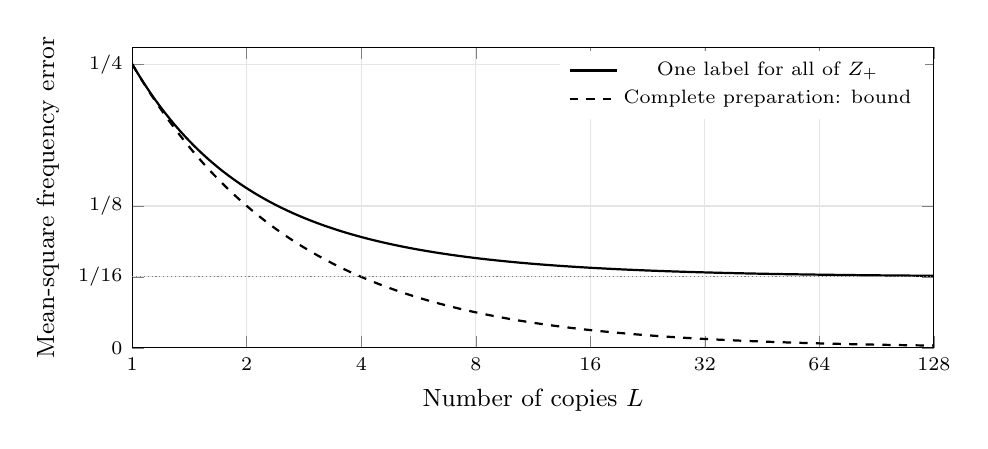
\begin{tikzpicture}
\begin{axis}[
 width=.97\columnwidth,height=5.4cm,
 xlabel={Number of copies $L$},ylabel={Mean-square frequency error},
 xmode=log,log basis x=2,xmin=1,xmax=128,ymin=0,ymax=.265,
 xtick={1,2,4,8,16,32,64,128},
 xticklabels={1,2,4,8,16,32,64,128},
 ytick={0,.0625,.125,.25},yticklabels={$0$,$1/16$,$1/8$,$1/4$},
 tick label style={font=\scriptsize},label style={font=\small},
 legend style={font=\scriptsize,draw=none,at={(.99,.99)},anchor=north east},
 grid=major,grid style={gray!20},clip=true]
\addplot[black,thick,domain=1:128,samples=170] {((x+1)/(4*x))^2};
\addlegendentry{One label for all of $Z_+$}
\addplot[black,dashed,thick,domain=1:128,samples=170] {1/(4*x)};
\addlegendentry{Complete preparation: bound}
\addplot[gray,densely dotted,domain=1:128] {1/16};
\end{axis}
\end{tikzpicture}
